\setcounter{section}{6}

\section{Синтаксичний аналіз в мовних процесорах}

\subsection{Синтаксичний аналіз}

Для визначення синтаксичної компоненти мови програмування використовують контекстно-вільні граматики (КС-граматики). На відміну від скінченно-автоматних граматик потужність класу КС-граматик достатня, щоб визначити майже всі так звані синтаксичні властивості мов програмування. Якщо цього недостатньо, то розглядають деякі спрощення у граматиках типу 2
або параметричні КC-граматики. \medskip

Звичайно, із синтаксичною компонентою мови програмування пов'язана семантична компонента. Тоді, якщо ми говоримо про семантику мови програмування, ми вимагаємо семантичної однозначності для кожної вірно написаної програми. За аналогією з семантикою, при описі синтаксичної компоненти мови програмування необхідно користуватися однозначними граматиками. \medskip

Граматика $G$ називається \textit{неоднозначною}, якщо існує декілька варіантів виводу $\omega$ в $G$ $\left(\omega \in L(G)\right)$. \medskip

\textbf{Приклад.} Розглянемо таку граматику $G = \left\langle N, \Sigma, P, S\right\rangle$ з двома правилами у схемі $P$: $S \Rightarrow S + S$, і $S \Rightarrow a$. Покажемо, що для ланцюжка $\omega = a + a + a$ існує щонайменше два варіанти виводу:
\begin{enumerate}
	\item $S \Rightarrow S + S \Rightarrow S + S + S \Rightarrow a + S + S \Rightarrow a + a + S \Rightarrow a + a + a$.
	\item $S \Rightarrow S + S \Rightarrow a + S \Rightarrow a + S + S \Rightarrow a + a + S \Rightarrow a + a + a$.
\end{enumerate}

\subsubsection{Стратегії виведення}

В теорії граматик розглядається декілька стратегій виведення ланцюжка $\omega$ в $G$. Визначимо дві стратегії які будуть використані в подальшому. \medskip\

\textit{Лівостороння стретегія виводу} ланцюжка $\omega$ в $G$ --- це послідовність кроків безпосереднього виводу, при якій на кожному кроці до увагі береться перший зліва направо нетермінал. \medskip

\textit{Правостороння стратегія виводу} $\omega$ в $G$ протилежна лівосторонній стратегії. \medskip

З виводом $\omega$ в $G$ пов'язане синтаксичне дерево, яке визначає синтаксичну структуру програми.

\subsubsection{Синтаксичні дерева}

\textit{Синтаксичне дерево виведення} $\omega$ в $G$ --- це впорядковане дерево, корінь котрого позначено аксіомою, в проміжних вершинах знаходяться нетермінали, а на кроні --- елементи з $\Sigma \cup \{\varepsilon\}$. Побудова синтаксичного дерева виведення $\omega$ в $G$ виконується покроково з урахуванням стратегії виводу $\omega$ в $G$. \medskip


\textbf{Алгоритм [побудови синтаксичного дерева ланцюжка $\omega$ в граматиці $G$ урахуванням лівосторонньої стратегії виводу].}
\begin{enumerate}
	\item Будуємо корінь дерева та позначимо його аксіомою $S$.

	\item В схемі $P$ граматики $G$ візьмемо правило виду $S \Rightarrow \alpha_1 \alpha_2 \ldots \alpha_p$, де $\alpha_i \in N \cup \Sigma \cup \{\varepsilon\} $	і побудуємо дерево висоти 1: 
	\begin{figure}[H]
		\centering
		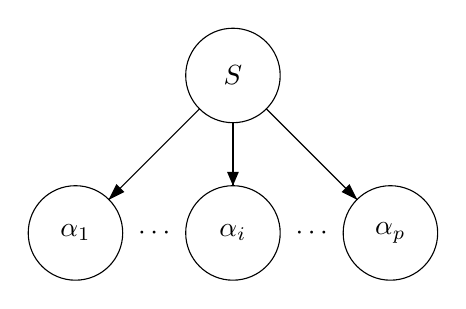
\begin{tikzpicture}[scale=0.2]
\tikzstyle{every node}+=[inner sep=0pt]
\draw [black] (0,0) circle (3);
\draw (0,0) node {$S$};

\draw [black] (-2.1, -2.1) -- (-7.9, -7.9);
\fill [black] (-7.9, -7.9) -- (-6.9, -7.4) -- (-7.4, -6.9);
\draw [black] (-10, -10) circle (3);
\draw (-10, -10) node {$\alpha_1$};

\draw (-5, -10) node {$\cdots$};

\draw [black] (0, -3) -- (0, -7);
\fill [black] (0, -7) -- (-.375, -6.125) -- (+.375, -6.125);
\draw [black] (0, -10) circle (3);
\draw (0, -10) node {$\alpha_i$};

\draw (+5, -10) node {$\cdots$};

\draw [black] (+2.1, -2.1) -- (+7.9, -7.9);
\fill [black] (+7.9, -7.9) -- (+6.9, -7.4) -- (+7.4, -6.9);
\draw [black] (+10, -10) circle (3);
\draw (+10, -10) node {$\alpha_p$};
\end{tikzpicture}

	\end{figure}

	\item На кроні дерева, побудованого на попередньому кроці, візьмемо перший зліва направо нетермінал. Нехай це буде $\alpha_i$. Тоді в схемі $P$ виберемо правило виду $\alpha_i \Rightarrow \beta_1 \beta_2 \ldots \beta_l$, де $\beta_i \in N \cup \Sigma \cup \{\varepsilon\}$ і побудуємо наступне дерево: 
	\begin{figure}[H]
		\centering
		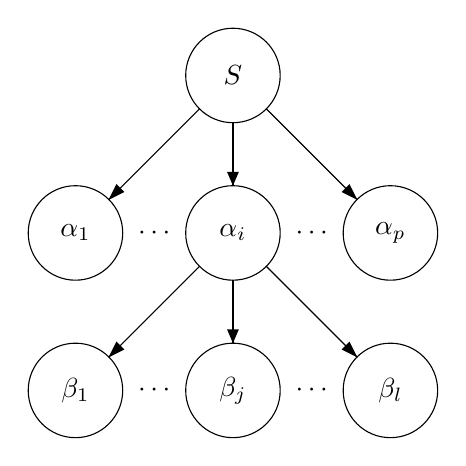
\begin{tikzpicture}[scale=0.2]
\tikzstyle{every node}+=[inner sep=0pt]
\draw [black] (0,0) circle (3);
\draw (0,0) node {$S$};

\draw [black] (-2.1, -2.1) -- (-7.9, -7.9);
\fill [black] (-7.9, -7.9) -- (-6.9, -7.4) -- (-7.4, -6.9);
\draw [black] (-10, -10) circle (3);
\draw (-10, -10) node {$\alpha_1$};

\draw (-5, -10) node {$\cdots$};

\draw [black] (0, -3) -- (0, -7);
\fill [black] (0, -7) -- (-.375, -6.125) -- (+.375, -6.125);
\draw [black] (0, -10) circle (3);
\draw (0, -10) node {$\alpha_i$};

\draw (+5, -10) node {$\cdots$};

\draw [black] (+2.1, -2.1) -- (+7.9, -7.9);
\fill [black] (+7.9, -7.9) -- (+6.9, -7.4) -- (+7.4, -6.9);
\draw [black] (+10, -10) circle (3);
\draw (+10, -10) node {$\alpha_p$};

\draw [black] (-2.1, -12.1) -- (-7.9, -17.9);
\fill [black] (-7.9, -17.9) -- (-6.9, -17.4) -- (-7.4, -16.9);
\draw [black] (-10, -20) circle (3);
\draw (-10, -20) node {$\beta_1$};

\draw (-5, -20) node {$\cdots$};

\draw [black] (0, -13) -- (0, -17);
\fill [black] (0, -17) -- (-.375, -16.125) -- (+.375, -16.125);
\draw [black] (0, -20) circle (3);
\draw (0, -20) node {$\beta_j$};

\draw (+5, -20) node {$\cdots$};

\draw [black] (+2.1, -12.1) -- (+7.9, -17.9);
\fill [black] (+7.9, -17.9) -- (+6.9, -17.4) -- (+7.4, -16.9);
\draw [black] (+10, -20) circle (3);
\draw (+10, -20) node {$\beta_l$};
\end{tikzpicture}

	\end{figure}

	Цей крок виконується доки на кроні дерева є елементи з $N$.
\end{enumerate}

Зауважимо очевидні факти, що випливають з побудови синтаксичного дерева:
\begin{itemize}
	\item крона дерева, зображеного на попередньому малюнку наступна:
	\begin{equation}
		\alpha_1 \alpha_2 \ldots \alpha_{i - 1} \beta_1 \beta_2 \ldots \beta_l \alpha_{i + 1} \ldots \alpha_p;
	\end{equation}
	\item ланцюжок $\alpha_1 \alpha_2 \ldots \alpha_{i - 1} \in \Sigma^\star$ з крони --- термінальний ланцюжок;
	\item для однозначної граматики $G$ існує лише одне синтаксичне дерево виводу $\omega$ в $G$.
\end{itemize}

\subsubsection{Власне аналіз}

Будемо говорити, що ланцюжок $\omega \in \Sigma^\star$, побудований на основі граматики $G$ $\left(\omega \in L(G)\right)$ \textit{проаналізований}, якщо відоме одне з його дерев виводу. \medskip

Зафіксуємо послідовність номерів правил, які були використані під час побудови синтаксичного дерева виводу $\omega$ в $G$ з урахуванням стратегії виводу. \medskip

\textit{Лівостороннім аналізом} $\pi$ ланцюжка $\omega \in L(G)$ будемо називати послідовність номерів правил, які були використані при лівосторонньому виводі $\omega$ в $G$. \medskip

\textbf{Приклад:} Для граматики $G = \left\langle N, \Sigma, P, S\right\rangle$ зі схемою $P$:
\begin{align}
	S &\Rightarrow S + T \\
	S &\Rightarrow T \\
	T &\Rightarrow T \times F \\
	T &\Rightarrow F \\
	F &\Rightarrow (S) \\
	F &\Rightarrow a
\end{align}
і для ланцюжка $\omega = a \times (a + a)$ побудуємо лівосторонній аналіз $\pi$: \medskip

Виведення має вигляд:
\begin{multline*}
	S \Rightarrow T \Rightarrow T \times F \Rightarrow F \times F \Rightarrow a \times F \Rightarrow a \times (S) \Rightarrow a \times (S + T) \Rightarrow \\
	\Rightarrow a \times (T + T) \Rightarrow a \times (F + T) \Rightarrow a \times (a + T) \Rightarrow a \times (a + F) \Rightarrow a \times (a + a).
\end{multline*}

З наведеного вище виводу ланцюжка $\omega \in L(G)$ лівосторонній аналіз $\pi$ буде: $\pi = (2, 3, 4, 6, 5, 1, 2, 4, 6, 4, 6)$, а синтаксичне дерево виводу $\omega = a \times (a + a)$ наступне:
\begin{figure}[H]
	\centering
	\setcounter{section}{11}

\section{Побудова $LL(k)$-синтаксичного аналізатора}

\subsection{Побудова $LL(k)$-синтаксичного аналізатора}

Повернемось до умови, при якій граматика $G$ буде $LL(k)$-граматикою, а саме: для довільного виведення $S \Rightarrow^\star \omega_1 A \omega_2$ та правила $A \mapsto \alpha \mid \beta$ маємо $\text{First}_l(\alpha \cdot L) \cap \text{First}_k(\beta \cdot L) = \varnothing$, де $L = \text{First}_k(\omega_2)$. \medskip

Оскільки $L \subseteq \Sigma^{\star k}$ --- конструктивна множина, спробуємо побудувати всілякі множини $L$, які задовольняють попередньо сформульованій умові.

\subsubsection{$\text{Local}_k(S, A)$}

Визначимо наступну множину:
\[\text{Local}_k(S, A) = \left\{ L \mid \exists x, \omega: S \Rightarrow^\star xA\omega, L = \text{First}_k(\omega) \right\}\]

Опишемо алгоритм пошуку цієї множини:
\begin{enumerate}
\item $\delta_0(S, S) = \{\{\varepsilon\}\}$, в інших випадках --- невизначено.
\item $\delta_1(S, A_i) = \delta_0(S, A_i) \cup \left\{ L \mid S \mapsto \omega_1 A_i \omega_2, L = \text{First}_k (\omega_2) \right\}$, в інших випадках --- невизначено.
\item 
\begin{multline*}
	\delta_n(S, A_i) = \delta_{n - 1}(S, A_i) \cup \\
	\cup \left\{ L \mid A_j \mapsto \omega_1 A_i \omega_2, L = \text{First}_k (\omega_2) \oplus_k L_p, L_p \in \text{Local}_k(S, A_j) \right\},
\end{multline*}
в інших випадках --- невизначено.
\item $\delta_m(S, A_i) = \delta_{m + 1}(S, A_i) = \ldots$, $\forall A_i \in N$.
\end{enumerate}

Тоді $\text{Local}_k(S, A_i) = \delta_m(S, A_i)$. \medskip

Виходячи з означення $\text{Local}_k(S, A_i)$, умови для $LL(k)$-граматики будуть наступними: для довільного $A$-правила вигляду $A \mapsto \omega_1 \mid \omega_2 \mid \ldots \mid \omega_p$ маємо: \[\text{First}_k (\omega_i \cdot L_m) \cap \text{First}_k(\omega_j \cdot L_m) = \varnothing, \quad i \ne k, \quad L_m \in \text{Local}_k(S, A).\]

Як наслідок, з алгоритму пошуку $\text{Local}_k(S, A_i)$ видно, що \[ \text{Follow}_k(A_i) = \bigcup_{j = 1}^m L_j, \quad L_j \in \text{Local}_k(S, A_i).\]

\subsubsection{Таблиці керування}

Для побудови синтаксичного аналізатора для $LL(k)$-граматики $(k > 1)$ необхідно побудувати множину таблиць, що забезпечать нам безтупиковий аналіз вхідного ланцюжка $w$ (програми) за час $O(n)$, де $n = \vert w\vert$. \medskip

Побудову множини таблиць для управління $LL(k)$-аналізатором почнемо з таблиці, яка визначає перший крок безпосереднього виводу $w$ в граматиці $G$: $T_0 = T_{S, \{\varepsilon\}}(u) = (T_1\alpha_1T_2\alpha_2\ldots T_p\alpha_p, n)$, де $n$ --- номер правила вигляду $S\mapsto A_1\alpha_1A_2\alpha_2\ldots Ap\alpha_p$, а $A_i \in N$, $\alpha_i \in \Sigma^\star$, і $u = \text{First}_k(A_1\alpha_1A_2\alpha_2\ldots A_p\alpha_p)$, і нарешті $i = \overline{1..p}$. Зрозуміло, що в інших випадках (якщо такого правила немає абощо) $T_0$ не визначена. \medskip

Неформально, коли в магазині автомата знаходиться аксіома $S$, то нас цікавить перших $k$ термінальних символів, які можна вивести з $S$ (аксіома --- поняття ``програма'') при умові, що після неї (програми) буде досягнуто EOF. \medskip

Імена інших таблиць $T_1, T_2, \ldots, T_p$ визначаються так: $T_i = T_{A_i, L_i}$, де $L_i = \text{First}_k(\alpha_i A_{i + 1} \alpha_{i + 1} \ldots A_p \alpha_p)$, $i = \overline{1..p}$. \medskip

Наступні таблиці визначаються так: $T_i = T_{A_i, L_i}(u) = (T_1\alpha_1T_2\alpha_2\ldots T_p\alpha_p, n)$, де $n$ --- номер правила вигляду $A_i\mapsto A_1\alpha_1A_2\alpha_2\ldots Ap\alpha_p$, а $A_j \in N$, $\alpha_j \in \Sigma^\star$, і $u = \text{First}_k(A_1\alpha_1A_2\alpha_2\ldots A_p\alpha_p) \oplus_k L_i$, і нарешті $j = \overline{1..p}$. Зрозуміло, що в інших випадках (якщо такого правила немає абощо) $T_i$ не визначена. \medskip

Імена інших таблиць $T_1, T_2, \ldots, T_p$ визначаються так: $T_j = T_{A_j, L_j}$, де $L_j = \text{First}_k(\alpha_j A_{j + 1} \alpha_{j + 1} \ldots A_p \alpha_p) \oplus_k L_i$, $j = \overline{1..p}$.

\subsubsection{Приклад}

Побудувати множину таблиць управління для $LL(2)$-граматики з наступною схемою правил:
\setcounter{equation}{0}
\begin{align}
	S &\mapsto abA, \\
	S &\mapsto \varepsilon, \\
	A &\mapsto Saa, \\
	A &\mapsto b.
\end{align}

Для вищенаведеної граматики множини $\text{First}_2(A_i)$, $A_i \in N$ будуть такі: $\text{First}_2(S) = \{ab, \varepsilon\}$, $\text{First}_2(A) = \{aa, ab, b\}$, а множини $\text{Local}_2(S, A_i)$, $A_i \in N$ будуть такі: $\text{Local}_2(S, S) = \text{Local}_2(S, A) = \{\{\varepsilon\}, \{aa\}\}$. \medskip

Побудуємо першу таблицю $T_0 = T_{S, \{\varepsilon\}}$. Для $S$-правила відповідні множини $u$ будуть такі:
\begin{itemize}
	\item $S \mapsto abA$, $u \in \text{First}_2(abA) = \{ab\}$.
	\item $S \mapsto \varepsilon$, $u \in \text{First}_2(\varepsilon) = \{\varepsilon\}$.
\end{itemize}

Таблиця $T_0$ визначається так:
\begin{table}[H]
	\centering
	\begin{tabular}{|c|c|c|c|c|c|c|c|}
		\hline
		& $aa$ & $ab$ & $ba$ & $bb$ & $a$ & $b$ & $\varepsilon$ \\ \hline
		$T_0 = T_{S, \{\varepsilon\}}$ &  & $abT_1$, 1 &  &  &  &  & $\varepsilon$, 2 \\ \hline
	\end{tabular}
\end{table}

Нова таблиця управління $T_1 = T_{A, \{\varepsilon\}}$. Для $A$-правила відповідні множини $u$ будуть такі:
\begin{itemize}
	\item $A \mapsto Saa$, $u \in \text{First}_2(Saa) \oplus_2 \{\varepsilon\} = \{ab, aa\}$.
	\item $A \mapsto b$, $u \in \text{First}_2(b) \oplus_2 \{\varepsilon\} = \{b\}$.
\end{itemize}

Таблиця $T_1$ визначається так:
\begin{table}[H]
	\centering
	\begin{tabular}{|c|c|c|c|c|c|c|c|}
		\hline
		 & $aa$ & $ab$ & $ba$ & $bb$ & $a$ & $b$ & $\varepsilon$ \\ \hline
		$T_1 = T_{A, \{\varepsilon\}}$ & $T_2aa$, 3 & $T_2aa$, 3 &  &  &  & $b$, 4 &  \\ \hline
	\end{tabular}
\end{table}

Нова таблиця управління $T_2 = T_{S, L}$ де $L = \text{First}_2 (aa) \oplus_2 \{\varepsilon\} = \{aa\}$. Для таблиці $T_2$ та $S$-правила множини $u$ будуть такі
\begin{itemize}
	\item $S \mapsto abA$, $u \in \text{First}_2(abA) \oplus_2 \{aa\} = \{ab\} \oplus_2 \{aa\} = \{ab\}$.
	\item $S \mapsto \varepsilon$, $u \in \text{First}_2(\varepsilon) \oplus_2 \{aa\} = \{aa\}$.
\end{itemize}

\begin{table}[H]
	\centering
	\begin{tabular}{|c|c|c|c|c|c|c|c|}
		\hline
		 & $aa$ & $ab$ & $ba$ & $bb$ & $a$ & $b$ & $\varepsilon$ \\ \hline
		$T_2 = T_{S, \{aa\}}$ & $\varepsilon$, 2 & $abT_3$, 1 &  &  &  &  &  \\ \hline
	\end{tabular}
\end{table}

Наступна таблиця $T_3 = T_{A, L}$ де $L = \text{First}_2(\varepsilon) \oplus_2 \{aa\} = \{aa\}$. Для таблиці $T_3$ та $A$-правила множини $u$ будуть такі:
\begin{itemize}
	\item $A \mapsto Saa$, $u \in \text{First}_2(Saa) \oplus_2 \{aa\} = \{ab, aa\}$.
	\item $A \mapsto b$, $u \in \text{First}_2(b) \oplus_2 \{aa\} = \{ba\}$.
\end{itemize}

Таблиця $T_3$ визначається так:
\begin{table}[H]
	\centering
	\begin{tabular}{|c|c|c|c|c|c|c|c|}
		\hline
		 & $aa$ & $ab$ & $ba$ & $bb$ & $a$ & $b$ & $\varepsilon$ \\ \hline
		$T_3 = T_{A, \{aa\}}$ & $T_2aa$, 3 & $T_2aa$, 3 & $b$, 4 &  &  &  &  \\ \hline
	\end{tabular}
\end{table}

Нова таблиця $T_4 = T_{S, L} = T_2$, оскільки $L = \text{First}_2(aa) \oplus_2 \{aa\} = \{aa\}$. \medskip

Ми визначили чотири таблиці-рядки (а їх кількість для довільної $LL(k)$-граматики визначається як $\sum_{i = 1}^n n_i$, де $n_i$ --- кількість елементів множини $\text{Local}_k(S, A_i)$, $m = \vert N\vert$. \medskip

Об'єднаємо рядки-таблиці в єдину таблицю та виконаємо перейменування рядків:

\begin{table}[H]
	\centering
	\begin{tabular}{|c|c|c|c|c|c|c|c|}
		\hline
		 & $aa$ & $ab$ & $ba$ & $bb$ & $a$ & $b$ & $\varepsilon$ \\ \hline
		$T_0$ &  & $abT_1$, 1 &  &  &  &  & $\varepsilon$, 2 \\ \hline
		$T_1$ & $T_2aa$, 3 & $T_2aa$, 3 &  &  &  & $b$, 4 &  \\ \hline
		$T_2$ & $\varepsilon$, 2 & $abT_3$, 1 &  &  &  &  &  \\ \hline
		$T_3$ & $T_2aa$, 3 & $T_2aa$, 3 & $b$, 4 &  &  &  &  \\ \hline
	\end{tabular}
\end{table}
\subsubsection{Алгоритм}

Синтаксичний аналізатор для $LL(k)$-граматики $(k > 1)$.
\begin{enumerate}
	\item Прочитати $k$ лексем з вхідного файла програми (звичайно, інколи менше ніж $k$). В магазин занести таблицю $T_0$.
	\item Загальний крок:
	\begin{itemize}
		\item Якщо на вершині магазина знаходиться таблиця $T_i$, то елемент таблиці $M(T_i, \langle \text{k вхідних лексем}\rangle)$ визначає ланцюжок, який $T_i$ заміщає на вершині магазина.
		\item Якщо на вершині магазина $a_i \in \Sigma$ перша поточна лексема з $k$ прочитаних лексем рівна $a_i$, то з вершини магазина зняти $a_i$ та прочитати з вхідного файла додатково одну лексему (звичайно, якщо це можливо).
		\item Якщо досягли кінця вхідного файла програми та магазин порожній, то програма не має синтаксичних помилок.
		\item В інших випадках --- синтаксична помилка.
	\end{itemize}
\end{enumerate}

\subsection{Контрольні запитання}
\begin{enumerate}
	\item Наведіть визначення множини $\text{Local}_k(S, A)$.
	\item Опишіть алгоритм побудови $\text{Local}_k(S, A)$.
	\item Опишіть алгоритм побудови таблиць керування (або рядків великої результуючої таблиці керування).
	\item Якою формулою визначається кількість рядків таблиці керування?
	\item Опишіть алгоритм синтаксичного аналізу для $LL(k)$-граматики.
\end{enumerate}

\end{figure}

\subsubsection{Синтез дерева за аналізом}

Нехай $\pi$ --- лівосторонній аналіз ланцюжка $\omega \in L(G)$. Знаючи $\pi$ досить легко побудувати (відтворити) синтаксичне дерево. Відтворення (синтез) синтаксичного дерева можна виконати, скориставшись однією з стратегій синтаксичного аналізу:
\begin{itemize}
	\item стратегія ``зверху донизу'';
	\item стратегія ``знизу догори''.
\end{itemize}

Стратегія синтаксичного аналізу \textit{``зверху донизу''} --- це побудова синтаксичного дерева крок за кроком починаючи від кореня до крони. \medskip

\textbf{Алгоритм [синтезу синтаксичного дерева на основі лівостороннього аналізу $\pi$ ланцюжка $\omega \in L(G)$].}
\begin{enumerate}
	\item Побудуємо корінь дерева та позначимо його аксіомою $S$. Тоді, якщо $\pi = (p_1, p_2, \ldots, p_m)$, то

	\item Побудуємо дерево висоти один, взявши зі схеми $P$ правило з номером $p_1$ виду $S \Rightarrow \alpha_1 \alpha_2 \ldots \alpha_p$:
	\begin{figure}[H]
		\centering
		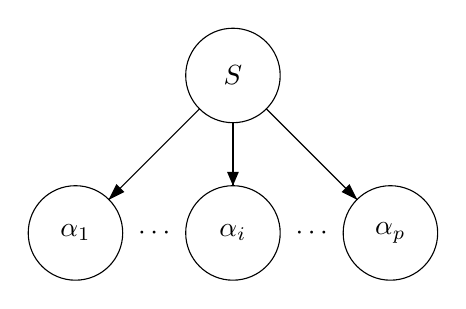
\begin{tikzpicture}[scale=0.2]
\tikzstyle{every node}+=[inner sep=0pt]
\draw [black] (0,0) circle (3);
\draw (0,0) node {$S$};

\draw [black] (-2.1, -2.1) -- (-7.9, -7.9);
\fill [black] (-7.9, -7.9) -- (-6.9, -7.4) -- (-7.4, -6.9);
\draw [black] (-10, -10) circle (3);
\draw (-10, -10) node {$\alpha_1$};

\draw (-5, -10) node {$\cdots$};

\draw [black] (0, -3) -- (0, -7);
\fill [black] (0, -7) -- (-.375, -6.125) -- (+.375, -6.125);
\draw [black] (0, -10) circle (3);
\draw (0, -10) node {$\alpha_i$};

\draw (+5, -10) node {$\cdots$};

\draw [black] (+2.1, -2.1) -- (+7.9, -7.9);
\fill [black] (+7.9, -7.9) -- (+6.9, -7.4) -- (+7.4, -6.9);
\draw [black] (+10, -10) circle (3);
\draw (+10, -10) node {$\alpha_p$};
\end{tikzpicture}

	\end{figure}

	\item На кроні дерева, отриманого на попередньому кроку, візьмемо перший зліва направо нетермінал (нехай це буде нетермінал $\alpha_i$) та правило з номером $p_j$ вигляду: $\alpha_i \Rightarrow \beta_1 \beta_2 \ldots \beta_l$ та побудуємо нове дерево:
	\begin{figure}[H]
		\centering
		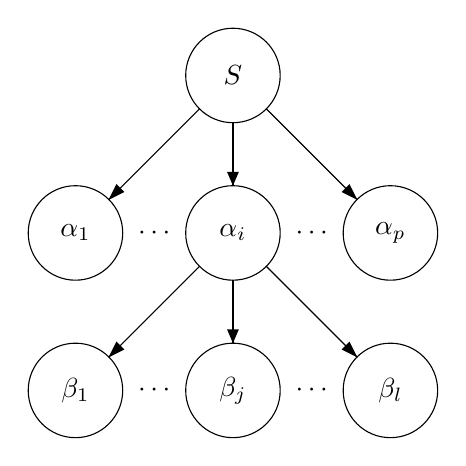
\begin{tikzpicture}[scale=0.2]
\tikzstyle{every node}+=[inner sep=0pt]
\draw [black] (0,0) circle (3);
\draw (0,0) node {$S$};

\draw [black] (-2.1, -2.1) -- (-7.9, -7.9);
\fill [black] (-7.9, -7.9) -- (-6.9, -7.4) -- (-7.4, -6.9);
\draw [black] (-10, -10) circle (3);
\draw (-10, -10) node {$\alpha_1$};

\draw (-5, -10) node {$\cdots$};

\draw [black] (0, -3) -- (0, -7);
\fill [black] (0, -7) -- (-.375, -6.125) -- (+.375, -6.125);
\draw [black] (0, -10) circle (3);
\draw (0, -10) node {$\alpha_i$};

\draw (+5, -10) node {$\cdots$};

\draw [black] (+2.1, -2.1) -- (+7.9, -7.9);
\fill [black] (+7.9, -7.9) -- (+6.9, -7.4) -- (+7.4, -6.9);
\draw [black] (+10, -10) circle (3);
\draw (+10, -10) node {$\alpha_p$};

\draw [black] (-2.1, -12.1) -- (-7.9, -17.9);
\fill [black] (-7.9, -17.9) -- (-6.9, -17.4) -- (-7.4, -16.9);
\draw [black] (-10, -20) circle (3);
\draw (-10, -20) node {$\beta_1$};

\draw (-5, -20) node {$\cdots$};

\draw [black] (0, -13) -- (0, -17);
\fill [black] (0, -17) -- (-.375, -16.125) -- (+.375, -16.125);
\draw [black] (0, -20) circle (3);
\draw (0, -20) node {$\beta_j$};

\draw (+5, -20) node {$\cdots$};

\draw [black] (+2.1, -12.1) -- (+7.9, -17.9);
\fill [black] (+7.9, -17.9) -- (+6.9, -17.4) -- (+7.4, -16.9);
\draw [black] (+10, -20) circle (3);
\draw (+10, -20) node {$\beta_l$};
\end{tikzpicture}

	\end{figure}

	Даний пункт виконувати доти, доки не переглянемо всі елементи з $\pi$.
\end{enumerate}

\subsubsection{Проблеми стратегії ``зверху донизу''}

Сформулюємо декілька проблему для стратегії аналізу ``зверху донизу'': \medskip

У загальному випадку у класі КС-граматик існує проблема неоднозначності (недетермінізму) виводу $\omega \in L(G)$. Як приклад можемо розглянути граматику з ``циклами''. Це така граматика, у якої в схемі $P$ існує така послідовність правил за участю нетермінала $A_i$, що: $A_i \Rightarrow A_j$ і $A_j \Rightarrow A_i$, де $A_j$ --- будь-який нетермінал граматики $G$. \medskip

Як наслідок, граматики з ліворекурсивним нетерміналом для стратегії аналізу ``зверху донизу'' недопустимі. \medskip % це ж чому? 

Зауважимо, що існують підкласи класу КС-граматик, які природно забезпечують стратегію аналізу ``зверху донизу''. Один з таких підкласів --- це $LL(k)$-граматики, які забезпечують синтаксичний аналіз ланцюжка $\omega \in L(G)$ за час $O(n)$, де $n = \vert \omega \vert$, та при цьому аналіз є однозначним.

\subsection{Контрольні запитання}

\begin{enumerate}
	\item Які граматики називаються однозначними? % не неоднозначні, тобто ті в яких у довільного ланцюжка не більше одного виведення
	\item Які дві стратегії виведення ви знаєте? % право- і ліво-стороння
	\item Що таке синтаксичне дерево виведення? % кроінь аксіома, з вершини стрілки у вершини що отримуються з неї безпосереднім виведенням...
	\item Що таке лівосторонній аналіз ланцюжка? % послідовність номерів правил схеми граматики викристаних при виведенні
	\item Що таке синтез дерева за аналізом? % процес побудоваи синтаксичного дерева виведення ланцюжка за синтаксичним аналізом цього ланцюжка
	\item Які дві стратегії синтезу дерева за аналізом ви знаєте? % зверху донизу і знизу догори
	\item Що таке граматика з циклами і які проблеми вона створює для стратегії ``згори донизу''? % граматика у схемі якої є правила $A_i \Rightarrow A_j \Rightarrow A_i$, вона призводить до неоднозначності виведення
	\item Який підклас КС-граматик забезпечує стратегію аналізу ``зверху донизу''? % LL(k), ми скоро визначимо цей підклас
\end{enumerate}
